\section{การซ่อมแซมภาพจิตรกรรมไทยโบราณ}
\hspace{1cm} สำหรับการซ่อมแซมจิตรกรรมไทยโบราณ ผู้วิจัยจะเริ่มจากการทำการปรับปรุงขั้นตอนวิธีเชิงตัวเลขที่มีอยู่แล้ว โดยใช้ภาพสีที่ได้สังเคราะห์ขึ้นทั้งสิ้น 5 ภาพ โดยแต่ละภาพมีขนาด 256 x 256 พิกเซล ดังรูปที่ \ref{figure:synart_original}

\begin{figure}[H]
    \centering
    \begin{subfigure}{\ResultSubFigureWidth \linewidth}
        \centering
        
\includegraphics[width=\ResultSubFigurePadding \linewidth]{image/image_inpaint_synthetic/case01-original.png}
    \end{subfigure}
    \begin{subfigure}{\ResultSubFigureWidth \linewidth}
        \centering
        
\includegraphics[width=\ResultSubFigurePadding \linewidth]{image/image_inpaint_synthetic/case02-original.png}
    \end{subfigure}
    \begin{subfigure}{\ResultSubFigureWidth \linewidth}
        \centering
        
\includegraphics[width=\ResultSubFigurePadding \linewidth]{image/image_inpaint_synthetic/case03-original.png}			
    \end{subfigure}
    \begin{subfigure}{\ResultSubFigureWidth \linewidth}
        \centering
        
\includegraphics[width=\ResultSubFigurePadding \linewidth]{image/image_inpaint_synthetic/case04-original.png}			
    \end{subfigure}
    \begin{subfigure}{\ResultSubFigureWidth \linewidth}
        \centering
        
\includegraphics[width=\ResultSubFigurePadding \linewidth]{image/image_inpaint_synthetic/case05-original.png}			
    \end{subfigure}
    \caption{ภาพต้นฉบับ}
    \label{figure:synart_original}
\end{figure}
\begin{figure}[H]
    \centering
    \begin{subfigure}{0.4\linewidth}
        \centering
        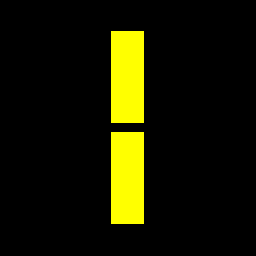
\includegraphics[width=0.8\linewidth]{image/image_inpaint_synthetic/case01-toinpaint.png}
    \end{subfigure}
    \begin{subfigure}{0.4\linewidth}
        \centering
        
\includegraphics[width=0.8\linewidth]{image/image_inpaint_synthetic/case02-toinpaint.png}
    \end{subfigure}
    \begin{subfigure}{0.4\linewidth}
        \centering
        
\includegraphics[width=0.8\linewidth]{image/image_inpaint_synthetic/case03-toinpaint.png}		
    \end{subfigure}
    \bigskip
    \begin{subfigure}{0.4\linewidth}
        \centering
        
\includegraphics[width=0.8\linewidth]{image/image_inpaint_synthetic/case04-toinpaint.png}		
    \end{subfigure}
    \begin{subfigure}{0.4\linewidth}
        \centering
        
\includegraphics[width=0.8\linewidth]{image/image_inpaint_synthetic/case05-toinpaint.png}		
    \end{subfigure}
    \caption{ภาพที่จะทำการซ่อมแซม}
\end{figure}

\subsection{การเปรียบเทียบประสิทธิภาพขั้นตอนวิธีเชิงตัวเลขที่มีอยู่แล้ว}
\hspace{1cm}
การทดสอบประสิทธิภาพจะใช้ $\varepsilon = 1 \times 10^{-4}$ และ $N= 10,000$ โดยรูปที่ \ref{figure:result-timemarching} - \ref{figure:result-splitbregman} และตารางที่ \ref{table:result-timemarching} - \ref{table:result-splitbregman} แสดงผลการซ่อมแซมภาพสังเคราะห์ทั้ง 5 ภาพ

\begin{figure}[H]
    \centering
    \begin{subfigure}{0.4\linewidth}
        \centering
        
\includegraphics[width=0.8\linewidth]{image/result_ex1/timemarch01.png}
    \end{subfigure}
    \begin{subfigure}{0.4\linewidth}
        \centering
        
\includegraphics[width=0.8\linewidth]{image/result_ex1/timemarch02.png}
    \end{subfigure}
    \begin{subfigure}{0.4\linewidth}
        \centering
        
\includegraphics[width=0.8\linewidth]{image/result_ex1/timemarch03.png}			
    \end{subfigure}
    \begin{subfigure}{0.4\linewidth}
        \centering
        
\includegraphics[width=0.8\linewidth]{image/result_ex1/timemarch04.png}			
    \end{subfigure}
    \begin{subfigure}{0.4\linewidth}
        \centering
        
\includegraphics[width=0.8\linewidth]{image/result_ex1/timemarch05.png}			
    \end{subfigure}
    \caption{ผลการซ่อมแซมจากวิธีการเดินเวลา}
    \label{figure:result-timemarching}
\end{figure}
\begin{table}[H]
	\centering
	\begin{tabular}[ht]{|c|c|c|c|c|}
		\hline
		รูปภาพ &เวลาประมวล  (วินาที) & PSNR (dB) & SSIM \\
		\hline
		1 & 82.40 & 25.17 & 0.9997 \\ 
		2 & 127.36 & 17.92 & 0.9980 \\
		3 &  116.39 & 13.33 & 0.9941 \\
		4 & 160.59  &12.40  & 0.9927 \\
		5 & 116.66  & 14.79  & 0.9958 \\
		\hline
		เฉลี่ย & 120.68  & 16.72  & 0.9960 \\
		\hline
	\end{tabular}
	\caption{ผลการซ่อมแซมวิธีการเดินเวลา}
	\label{table:result-timemarching}
\end{table}

\begin{figure}[H]
	\centering
	\begin{subfigure}{0.4\linewidth}
		\centering
		
\includegraphics[width=0.8\linewidth]{image/result_ex1/fixpoint01.png}
	\end{subfigure}
	\begin{subfigure}{0.4\linewidth}
		\centering
		
\includegraphics[width=0.8\linewidth]{image/result_ex1/fixpoint02.png}
	\end{subfigure}
	\begin{subfigure}{0.4\linewidth}
		\centering
		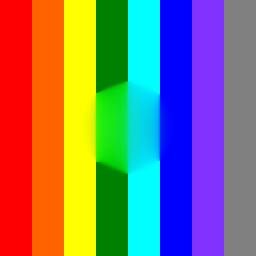
\includegraphics[width=0.8\linewidth]{image/result_ex1/fixpoint03.png}			
	\end{subfigure}
	\begin{subfigure}{0.4\linewidth}
		\centering
		
\includegraphics[width=0.8\linewidth]{image/result_ex1/fixpoint04.png}			
	\end{subfigure}
	\begin{subfigure}{0.4\linewidth}
		\centering
		
\includegraphics[width=0.8\linewidth]{image/result_ex1/fixpoint05.png}			
	\end{subfigure}
	\caption{ผลการซ่อมแซมจากวิธีการทำซ้ำแบบจุดตรึง}
\end{figure}
\begin{table}[H]
	\centering
	\begin{tabular}[ht]{|c|c|c|c|c|}
		\hline
		รูปภาพ &เวลาประมวล  (วินาที) & PSNR (dB) & SSIM \\
		\hline
		1 & 24.97 & 60.95 & 1.0000 \\ 
		2 & 53.06 & 37.69 & 1.0000 \\
		3 &  190.64 & 25.17 & 0.9997 \\
		4 & 50.63  & 28.81  & 0.9999 \\
		5 & 54.74  & 40.73  & 1.0000 \\
		\hline
		เฉลี่ย & 74.81  & 38.67  & 0.9999 \\
		\hline
	\end{tabular}
	\caption{ผลการซ่อมแซมของวิธีการทำซ้ำแบบจุดตรึง (Algorithm \ref{algorithm:fixedpoint})}
\end{table}	


\begin{figure}[H]
	\centering
	\begin{subfigure}{\ResultSubFigureWidth \linewidth}
		\centering
		
\includegraphics[width=\ResultSubFigurePadding \linewidth]{image/result_ex1/splitbergman01.png}
	\end{subfigure}
	\begin{subfigure}{\ResultSubFigureWidth \linewidth}
		\centering
		
\includegraphics[width=\ResultSubFigurePadding \linewidth]{image/result_ex1/splitbergman02.png}
	\end{subfigure}
	\begin{subfigure}{\ResultSubFigureWidth \linewidth}
		\centering
		
\includegraphics[width=\ResultSubFigurePadding \linewidth]{image/result_ex1/splitbergman03.png}			
	\end{subfigure}
	\begin{subfigure}{\ResultSubFigureWidth \linewidth}
		\centering
		
\includegraphics[width=\ResultSubFigurePadding \linewidth]{image/result_ex1/splitbergman04.png}			
	\end{subfigure}
	\begin{subfigure}{\ResultSubFigureWidth \linewidth}
		\centering
		
\includegraphics[width=\ResultSubFigurePadding \linewidth]{image/result_ex1/splitbergman05.png}			
	\end{subfigure}
	\caption{ผลการซ่อมแซมจากวิธีการสปริทเบรกแมน}
	\label{figure:result-splitbregman}
\end{figure}
\begin{table}[H]
	\centering
	\begin{tabular}[ht]{|c|c|c|c|c|}
		\hline
		รูปภาพ &เวลาประมวล  (วินาที) & PSNR (dB) & SSIM \\
		\hline
		1 & 3.39 & 71.54 & 1.0000 \\ 
		2 & 10.74 & 37.08 & 1.0000 \\
		3 &  24.50 & 26.08 & 0.9997 \\
		4 & 15.80  & 29.61  & 0.9999 \\
		5 & 15.85  & 32.78  & 1.0000 \\
		\hline
		เฉลี่ย & 14.06  & 39.42  & 0.9999 \\
		\hline
	\end{tabular}
	\caption{ผลการซ่อมแซมของวิธีสปริทเบรกแมน}
	\label{table:result-splitbregman}
\end{table}

\hspace{1cm} ประสิทธิภาพของวิธีการเชิงตัวเลขทั้ง 3 วิธี สามารถสรุปได้ดังนี้
\begin{table}[H]
    \centering
    \begin{tabular}[ht]{|l|c|c|c|c|}
        \hline
        วิธีการ  & เวลาประมวล  (วินาที) & PSNR (dB) & SSIM \\
        \hline
        วิธีเดินเวลา (Algorithm \ref{algorithm:explicit_timemarch})& 120.68 & 16.72 & 0.9960 \\
        วิธีทำซ้ำจุดตรึง (Algorithm \ref{algorithm:fixedpoint})& 74.81 & 38.67 & 0.9999 \\
        วิธีสปริทเบรกแมน (Algorithm \ref{algorithm:splitbregman}) & 14.06 & 39.42 & 0.9999  \\
        \hline
    \end{tabular}
    \caption{แสดงการซ่อมแซมเฉลี่ยของวิธีการเชิงตัวเลข}
\end{table}	
\hspace{1cm} 
จากทั้ง 3 วิธีที่ได้ทดสอบ จะเห็นได้ว่าวิธีการสปริทเบรกแมนใช้เวลาน้อยกว่าวิธีอื่น และมีคุณภาพ ซึ่งพิจารณาจาก ค่า PSNR และค่า SSIM มากกว่าวิธีอื่น ผู้วิจัยจึงสนใจทำการปรับปรุงวิธีสปิทเบรกแมนให้มีประสิทธิภาพสูง

\subsection{ขั้นตอนวิธีเชิงตัวเลขสำหรับต่อเติมภาพชนิดใหม่}

\hspace{1cm} ตารางที่ \ref{table:multiresolution} แสดงผลการเปรียบเทียบประสิทธิภาพของขั้นตอนวิธีการที่ \ref{algorithm:MultiSplitBregmanColorInpaint} ภายใต้การเปลี่ยนแปลงจำนวนรอบของการทำซ้ำของวิธีการสปริทเบรกแมนบนภาพที่มีความคมชัด 256x256 พิกเซล ตัวอย่าง เช่น 10/3/3/10000 หมายถึงที่ระดับความคมชัดหยาบสุดซึ่งมีขนาดเป็น 32x32 พิกเซลจะทำซ้ำไม่เกิน 10 ครั้ง สำหรับที่ความคมชัดละเอียดขึ้นเป็น 64x64 พิกเซลจะทำซ้ำไม่เกิน 3 ครั้ง และสำหรับที่ระดับความคมชัดเป็น 128x128 พิกเซลจะทำซ้ำ 3 ครั้ง และที่ระดับความคมชัดเป็น 256x256 จะทำซ้ำไม่เกิน 10,000 ครั้งหรือจนค่าความคลาดเคลื่อนสัมพัทธ์ต่างกันไม่เกิน 0.0001 
	
\begin{table}[H]
    \footnotesize
    \centering
    \begin{tabular}[ht]{|l|c|c|c|c|c|}
        \hline
        รูปแบบการทำซ้ำ  & รูปภาพ &เวลาประมวล  (วินาที) & PSNR (dB) & SSIM \\
        \hline
        ไม่ใช้พีระมิดรูปภาพ & 1 & 4.49  & 71.54 & 1.0000 \\ 
        & 2 & 13.16 & 37.08 & 1.0000 \\
        & 3 & 29.46 & 26.08 & 0.9997 \\
        & 4 & 20.50 & 29.61 & 0.9999 \\
        & 5 & 19.32 & 32.78 & 1.0000 \\
        \hline
        10/1/1/10000 & 1 & 2.44 & 69.59& 1.0000 \\
        & 2 & 11.31 &37.04 & 1.0000 \\
        & 3 & 23.48 & 27.34 & 0.9998 \\
        & 4 & 16.60 & 29.42 & 0.9999 \\
        & 5 & 13.75 & 33.53 & 1.0000 \\
        \hline
        10/3/3/10000  & 1 & 2.24 & 69.96 & 1.0000\\
        & 2 & 10.91 & 37.05 & 1.0000 \\
        & 3 & 21.99 & 27.66 & 0.9998 \\
        & 4 & 12.70 & 29.35 & 0.9999 \\
        & 5 & 11.49 & 33.69 & 1.0000\\
        \hline
        10/10/10/10000  & 1 & 1.83 & 71.58 & 1.0000 \\
        & 2 & 7.83 & 37.05 & 1.0000 \\
        & 3 & 16.75 & 28.62 & 0.9998 \\
        & 4 & 11.89 & 29.32 & 0.9999 \\
        & 5 & 8.00 & 34.26 & 1.0000 \\
        \hline
        100/1/1/10000  & 1 & 1.43 & 67.63 & 1.0000\\
        & 2 & 7.17 & 37.10 & 1.0000 \\
        & 3 & 20.86 & 27.70 & 0.9998 \\
        & 4 & 12.80 & 29.64 & 0.9999\\
        & 5 & 9.17 & 33.14 & 1.0000 \\
        \hline
        100/3/3/10000  & 1 & 1.68 & 71.18 & 1.0000 \\
        & 2 & 7.41 & 37.11 & 1.0000\\
        & 3 & 21.08 & 28.00 & 0.9998 \\
        & 4 & 13.28 & 29.38 & 0.9999 \\
        & 5 & 7.96 & 33.34 & 1.0000\\
        \hline
        100/10/10/10000  & 1 & 1.76 & 71.56 & 1.0000 \\
        & 2 & 7.32 & 37.04 & 1.0000\\
        & 3 & 16.62 & 28.65 & 0.9998 \\
        & 4 & 13.18 & 29.39 & 0.9999\\
        & 5 & 7.45 & 33.94 & 1.0000 \\
        \hline
    \end{tabular}
    \caption{ผลการซ่อมแซมภาพโดยวิธีการเชิงตัวเลขที่นำเสนอ}
    \label{table:multiresolution}
\end{table}	
\begin{table}[H]
    \centering
    \begin{tabular}[ht]{|l|c|c|c|c|}
        \hline
        รูปแบบการทำซ้ำ  & เวลาประมวล  (วินาที) & PSNR (dB) & SSIM \\
        \hline
        ไม่ใช้พีระมิดรูปภาพ & 17.38 & 39.42 & 0.9999 \\
        10/1/1/10000 & 13.52 & 39.38 & 0.9999 \\
        10/3/3/10000 & 11.86 & 39.54 & 0.9999 \\
        10/10/10/10000 & 9.26 & 40.17 & 0.9999\\
        100/1/1/10000 & 10.28 & 39.04 & 0.9999\\
        100/3/3/10000 & 10.28 & 39.80 & 0.9999\\
        100/10/10/10000 & 9.27 & 40.12 & 0.9999 \\
        \hline
    \end{tabular}
    \caption{ผลการซ่อมแซมภาพโดยวิธีการเชิงตัวเลขที่นำเสนอในรูปของค่าเฉลี่ยของผลที่ได้จากตารางที่ \ref{table:multiresolution}}
    \label{table:multiresolution-summary}
\end{table}	

\hspace{1cm}จากตารางที่ \ref{table:multiresolution-summary} สังเกตว่า ยิ่งจำนวนการทำซ้ำในชั้นที่รูปภาพมีขนาดเล็กจำนวนมากครั้ง จะยิ่งทำให้เวลาประมวลผลที่ใช้ในการต่อเติมภาพใช้เวลาน้อยลง

\hspace{1cm} นอกจากนี้แล้ว ผู้วิจัยยังได้สังเกตอีกว่า การทำซ้ำนั้นจะลู่เข้าเร็วในช่วงแรก จากนั้นความเร็วในการลู่เข้าจะลดลง ซึ่งทำให้การทำซ้ำเพียงไม่กี่ครั้งในระดับความคมชัดเดิม  มีผลการซ่อมแซมภาพจนแสดงความคล้ายคลึงกับภาพต้นฉบับได้

\hspace{1cm} ผู้วิจัยจึงกำหนดให้การทำซ้ำในระดับความละเอียดสุดเท่ากับ 10 ครั้ง และพบว่าได้ผลการซ่อมแซมดังตารางที่ \ref{table:multiresolution2}

\begin{table}[H]
	\centering
	\scalebox{0.8}{
	\begin{tabular}[ht]{|l|c|c|c|c|c|}
		\hline
		รูปแบบการทำซ้ำ  & รูปภาพ &เวลาประมวล  (วินาที) & PSNR (dB) & SSIM \\
		\hline
		ไม่ใช้พีระมิดรูปภาพ & 1 & 0.30  & 26.71  & 0.9998 \\ 
		& 2 & 0.39  & 18.39  & 0.9982 \\
		& 3 & 0.38 & 13.66  & 0.9944 \\
		& 4 & 0.40  & 12.86 & 0.9934 \\
		& 5 & 0.38 & 14.69 &  0.9956\\
		\hline
		10/1/1/10 & 1 & 0.29 & 40.10 & 1.0000\\
		& 2 & 0.41 & 31.28 & 0.9999 \\
		& 3 & 0.46 & 16.51 & 0.9970 \\
		& 4 & 0.47 & 26.56 & 0.9998\\
		& 5 & 0.39 & 28.25 & 0.9998 \\
		\hline
		10/3/3/10  & 1 & 0.28 & 42.53 & 1.0000\\
		& 2 & 0.36 & 32.91 & 1.0000 \\
		& 3 & 0.35 & 16.88 & 0.9972 \\
		& 4 & 0.34 & 27.06 &  0.9998 \\
		& 5 & 0.34 & 29.76 & 0.9999 \\
		\hline
		10/10/10/10  & 1 & 0.31 & 50.06 & 1.0000 \\
		& 2 & 0.41 & 34.01 & 1.0000\\
		& 3 & 0.38 & 18.19 & 0.9980\\
		& 4 & 0.39 & 27.50 & 0.9998\\
		& 5 & 0.40 & 33.05 &  1.0000\\
		\hline
		100/1/1/10  & 1 & 0.27 & 43.97 & 1.0000 \\
		& 2 & 0.37  & 31.28 & 0.9999\\
		& 3 & 0.36 & 24.98 & 0.9997\\
		& 4 & 0.36  &28.05 & 0.9998\\
		& 5 & 0.36 & 29.24 & 0.9999 \\
		\hline
		100/3/3/10  & 1 & 0.29 & 45.08& 1.0000 \\
		& 2 & 0.36 & 32.36 & 0.9999\\
		& 3 & 0.40 & 24.35 & 0.9996\\
		& 4 & 0.38 & 27.88 & 0.9998\\
		& 5 & 0.37 & 30.28 & 0.9999 \\
		\hline
		100/10/10/10  & 1 & 0.28 & 50.05 &  1.0000\\
		& 2 & 0.41 & 33.25 &  1.0000\\
		& 3 & 0.42 & 23.51 & 0.9995 \\
		& 4 & 0.42 & 27.78 & 0.9998 \\
		& 5 & 0.39 & 32.38 & 0.9999 \\
		\hline
	\end{tabular}
	}
	\caption{ผลการซ่อมแซมภาพโดยวิธีการเชิงตัวเลขที่นำเสนอเมื่อใช้การทำซ้ำในระดับความคมชัดละเอียดสุด 10 ครั้ง}
	\label{table:multiresolution2}
\end{table}	
\begin{table}[H]
    \centering
    \begin{tabular}[ht]{|l|c|c|c|c|}
        \hline
        รูปแบบการทำซ้ำ  & เวลาประมวล  (วินาที) & PSNR (dB) & SSIM \\
        \hline
        ไม่ใช้พีระมิดรูปภาพ & 0.37 & 17.26 & 0.9963  \\
        10/1/1/10 & 0.40 & 28.54 & 0.9993 \\
        10/3/3/10 & 0.33 & 29.83  & 0.9994 \\
        10/10/10/10 & 0.38 & 32.56 & 0.9995 \\
        100/1/1/10 & 0.34 & 31.50 & 0.9999 \\
        100/3/3/10 & 0.36 & 31.99 & 0.9999 \\
        100/10/10/10 & 0.38 & 33.39 & 0.9998 \\
        \hline
    \end{tabular}
    \caption{ผลการซ่อมแซมภาพโดยวิธีการเชิงตัวเลขที่นำเสนอในรูปของค่าเฉลี่ยของผลที่ได้จากตารางที่ \ref{table:multiresolution2}}
    \label{table:multiresolution2-summary}
\end{table}	

\hspace{1cm}จากตารางจะเห็นว่า การทำซ้ำในชั้นที่รูปภาพมีขนาดเล็กมากจำนวนมาก ไม่ช่วยให้การประมวลผลได้เร็วขึ้น ผู้วิจัยจึงเลือกใช้การทำซ้ำแบบ 10/3/3/10 ในการต่อเติมภาพ

\subsection{การทดสอบประสิทธิภาพในการซ่อมแซมภาพจิตรกรรมไทยโบราณ}

\hspace{1cm}ภาพจิตรกรรมทีี่ใช้ทดสอบ มีทั้งสิ้น 5  ภาพ โดยแต่ละภาพเป็นภาพสีที่มีขนาด 256x256 พิกเซล ซึ่งทั้ง 5 ภาพได้แก่ ภาพที่ \ref{image:thaiart_case01_original} \footnote{ภาพถ่ายที่วัดแก้วไพฑูรย์; ภาพจาก  https://commons.wikimedia.org/wiki/File:จิตรกรรมฝาผนัง\_วัดแก้วไพฑูรย์\_(7).jpg สืบค้นเมื่อวันที่ 23 กันยายน 2561}   และภาพที่ \ref{image:thaiart_case02_original} \footnote{ภาพถ่ายที่วัดแก้วไพฑูรย์; ภาพจาก  https://commons.wikimedia.org/wiki/File:จิตรกรรมฝาผนัง\_วัดแก้วไพฑูรย์\_(2).jpg สืบค้นเมื่อวันที่ 23 กันยายน 2561} คือ จิตรกรรมฝาผนังวัดแก้วไพฑูรย์ ภาพที่ \ref{image:thaiart_case03_original} \footnote{ภาพถ่ายที่วัดพระยืนพุทธบาทยุคล; ภาพจาก https://commons.wikimedia.org/wiki/File:Wat\_Phra\_Yuen \_Phutthabat\_Yukhon\_01.jpg สืบค้นเมื่อวันที่ 23 กันยายน 2561}  คือ จิตรกรรมฝาผนังวัดพระยืนพุทธบาทยุคล ภาพที่ \ref{image:thaiart_case04_original} \footnote{ภาพถ่ายที่วัดคงคาราม; ภาพจาก  https://commons.wikimedia.org/wiki/File:จิตรกรรม\_อุโบสถวัดคงคาราม.JPG สืบค้นเมื่อวันที่ 23 กันยายน 2561} คือ จิตรกรรมฝาผนังวัดคงคาราม และภาพที่ \ref{image:thaiart_case05_original} \footnote{ภาพถ่ายที่วัดท่าถนน; ภาพจาก  https://commons.wikimedia.org/wiki/File:Wat\_Tha\_Thanon\_05.JPG สืบค้นเมื่อวันที่ 23 กันยายน 2561} คือ จิตรกรรมฝาผนังวัดท่าถนน โดยจะทำให้ข้อมูลข้องทั้ง 5 ภาพเกิดความเสียหาย โดยใช้รอยความเสียหายจากภาพพระเจ้าสร้างอดัม
    
\begin{figure}[H]
    \centering
    \begin{subfigure}{\ResultSubFigureWidth \linewidth}
        \centering
        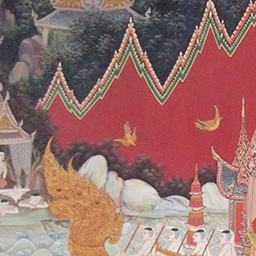
\includegraphics[width=\ResultSubFigurePadding \linewidth]{image/thaiart/case01-original.png}
        \caption{วัดแก้วไพฑูรย์}
        \label{image:thaiart_case01_original}
    \end{subfigure}
    \begin{subfigure}{\ResultSubFigureWidth \linewidth}
        \centering
        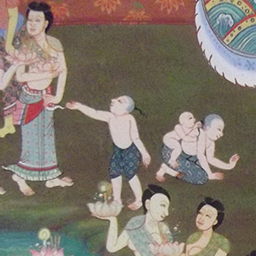
\includegraphics[width=\ResultSubFigurePadding \linewidth]{image/thaiart/case02-original.png}
        \caption{วัดแก้วไพฑูรย์}
        \label{image:thaiart_case02_original}
    \end{subfigure}
    \begin{subfigure}{\ResultSubFigureWidth \linewidth}
        \centering
        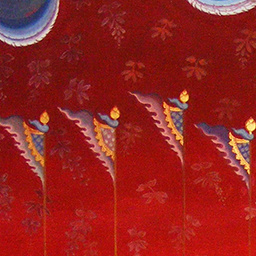
\includegraphics[width=\ResultSubFigurePadding \linewidth]{image/thaiart/case03-original.png}
        \caption{วัดพระยืนพุทธบาทยุคล}
        \label{image:thaiart_case03_original}			
    \end{subfigure}		
    \begin{subfigure}{\ResultSubFigureWidth \linewidth}
        \centering
        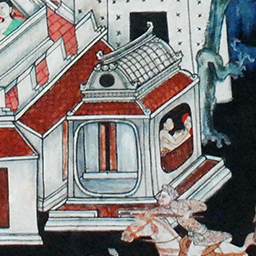
\includegraphics[width=\ResultSubFigurePadding \linewidth]{image/thaiart/case04-original.png}
        \caption{วัดคงคาราม}
        \label{image:thaiart_case04_original}			
    \end{subfigure}
    \begin{subfigure}{\ResultSubFigureWidth \linewidth}
        \centering
        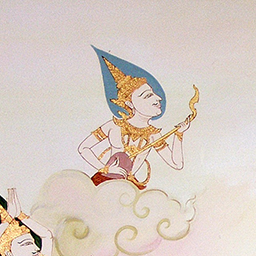
\includegraphics[width=\ResultSubFigurePadding \linewidth]{image/thaiart/case05-original.png}
        \caption{วัดท่าถนน}
        \label{image:thaiart_case05_original}			
    \end{subfigure}
    \begin{subfigure}{\ResultSubFigureWidth \linewidth}
        \centering
        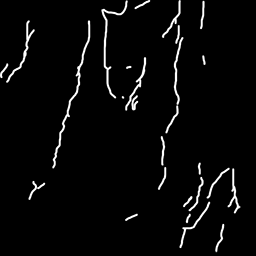
\includegraphics[width=\ResultSubFigurePadding \linewidth]{image/thaiart/inpaint-domain.png}
        \caption{รอยความเสียหาย}
    \end{subfigure}
    \caption{ภาพต้นฉบับสำหรับใช้ในการทดสอบ}
\end{figure}
\begin{figure}[H]
	\centering
	\begin{subfigure}{0.4\linewidth}
		\centering
		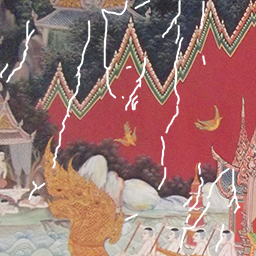
\includegraphics[width=0.8\linewidth]{image/thaiart/case01-toinpaint.png}
	\end{subfigure}
	\begin{subfigure}{0.4\linewidth}
		\centering
		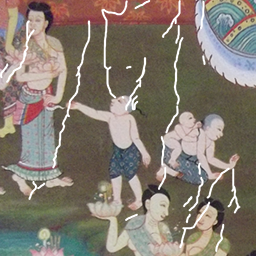
\includegraphics[width=0.8\linewidth]{image/thaiart/case02-toinpaint.png}
	\end{subfigure}
	\vspace{1cm}
	\begin{subfigure}{0.4\linewidth}
		\centering
		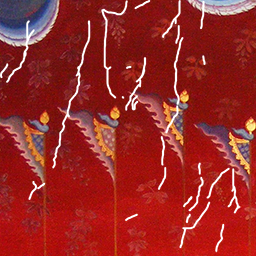
\includegraphics[width=0.8\linewidth]{image/thaiart/case03-toinpaint.png}			
	\end{subfigure}
	\begin{subfigure}{0.4\linewidth}
		\centering
		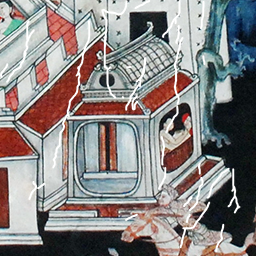
\includegraphics[width=0.8\linewidth]{image/thaiart/case04-toinpaint.png}			
	\end{subfigure}
	\begin{subfigure}{0.4\linewidth}
		\centering
		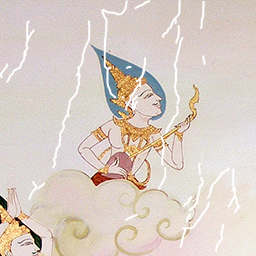
\includegraphics[width=0.8\linewidth]{image/thaiart/case05-toinpaint.png}			
	\end{subfigure}
	\caption{ภาพที่ทำให้เสียหาย}
\end{figure}

\hspace{1cm} จากนั้นทำการทดสอบการต่อเติมภาพทั้ง 5 โดยทดสอบวิธีสปริทเบรกแมน และวิธีทีที่พัฒนาขึ้นโดยใช้วิธีการสปริทเบรกแมนพร้อมทั้งการใช้พีระมิดรูปภาพที่มีการทำซ้ำแต่ละชั้นเป็น 10/3/3/10  ได้ผลลัพธ์ออกมาเป็นดังนี้

\begin{figure}[H]
    \centering
    \begin{subfigure}{0.4\linewidth}
        \centering
        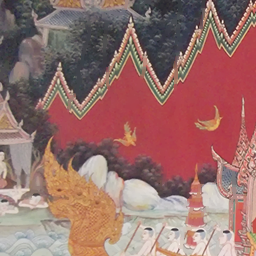
\includegraphics[width=0.8\linewidth]{image/result_ex4/splitbergman_case01.png}
    \end{subfigure}
    \begin{subfigure}{0.4\linewidth}
        \centering
        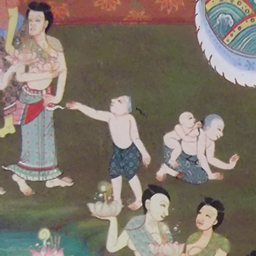
\includegraphics[width=0.8\linewidth]{image/result_ex4/splitbergman_case02.png}
    \end{subfigure}
    \begin{subfigure}{0.4\linewidth}
        \centering
        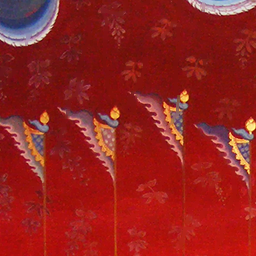
\includegraphics[width=0.8\linewidth]{image/result_ex4/splitbergman_case03.png}			
    \end{subfigure}
    \begin{subfigure}{0.4\linewidth}
        \centering
        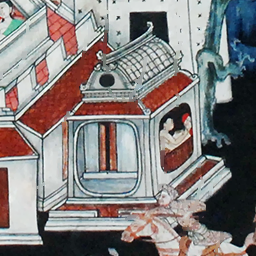
\includegraphics[width=0.8\linewidth]{image/result_ex4/splitbergman_case04.png}			
    \end{subfigure}
    \begin{subfigure}{0.4\linewidth}
        \centering
        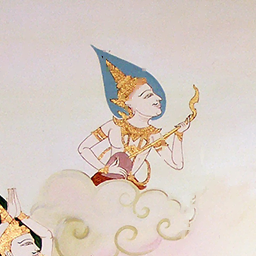
\includegraphics[width=0.8\linewidth]{image/result_ex4/splitbergman_case05.png}			
    \end{subfigure}
    \caption{ผลการซ่อมแซมโดยวิธีการสปริทเบรกแมน}
\end{figure}
\begin{table}[H]
    \centering
    \begin{tabular}[ht]{|c|c|c|c|c|}
        \hline
        รูปภาพ &เวลาประมวล  (วินาที) & PSNR (dB) & SSIM \\
        \hline
        1 & 2.95 & 33.92 & 1.0000 \\ 
        2 & 2.64 & 37.33 & 1.0000 \\
        3 &  3.49 & 37.21 & 1.0000 \\
        4 & 2.70  & 29.47  & 1.0000 \\
        5 & 15.85  & 32.78  & 1.0000 \\
        \hline
        เฉลี่ย & 2.72  & 34.89  & 1.0000 \\
        \hline
    \end{tabular}
    \caption{ผลการซ่อมแซมภาพศิลปะไทยจากวิธีการสปิทเบรกแมน}
    \label{table:ex4-splitbregman}
\end{table}

\begin{figure}[H]
    \centering
    \begin{subfigure}{0.4\linewidth}
        \centering
        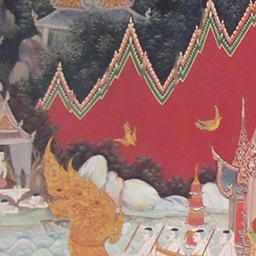
\includegraphics[width=0.8\linewidth]{image/result_ex4/multisplitbergman_case01.png}
    \end{subfigure}
    \begin{subfigure}{0.4\linewidth}
        \centering
        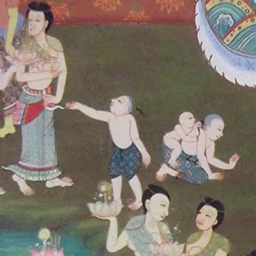
\includegraphics[width=0.8\linewidth]{image/result_ex4/multisplitbergman_case02.png}
    \end{subfigure}
    \begin{subfigure}{0.4\linewidth}
        \centering
        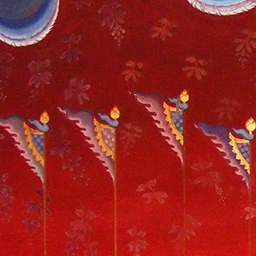
\includegraphics[width=0.8\linewidth]{image/result_ex4/multisplitbergman_case03.png}			
    \end{subfigure}
    \begin{subfigure}{0.4\linewidth}
        \centering
        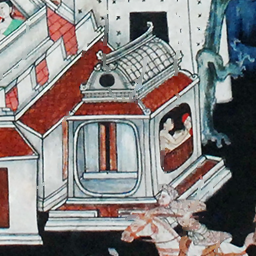
\includegraphics[width=0.8\linewidth]{image/result_ex4/multisplitbergman_case04.png}			
    \end{subfigure}
    \begin{subfigure}{0.4\linewidth}
        \centering
        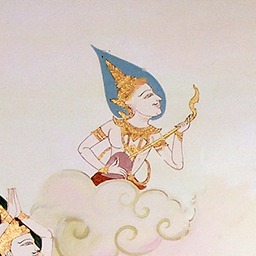
\includegraphics[width=0.8\linewidth]{image/result_ex4/multisplitbergman_case05.png}			
    \end{subfigure}
    \caption{ผลการซ่อมแซมภาพโดยวิธีการเชิงตัวเลขที่พัฒนาขึ้น}
\end{figure}
\begin{table}[H]
    \centering
    \begin{tabular}[ht]{|c|c|c|c|c|}
        \hline
        รูปภาพ &เวลาประมวล  (วินาที) & PSNR (dB) & SSIM \\
        \hline
        1 & 0.40 & 34.13 & 1.0000 \\ 
        2 & 0.40 & 38.18 & 1.0000 \\
        3 &  0.39 & 37.73 & 1.0000 \\
        4 & 0.38  & 29.38  & 1.0000 \\
        5 & 0.39  & 37.11  & 1.0000 \\
        \hline
        เฉลี่ย & 0.39  & 35.30  & 1.0000 \\
        \hline
    \end{tabular}
    \caption{ผลการซ่อมแซมภาพศิลปะไทยโดยวิธีการเชิงตัวเลขที่พัฒนาขึ้น}
    \label{table:ex4-multiresolution}
\end{table}	 

\hspace{1cm}ทั้งสองวิธี ได้ผลลัพธ์การซ่อมแซมภาพศิลปะไทยในรูปค่าเฉลี่ยออกมาดังนี้

\begin{table}[H]
    \centering
    \begin{tabular}[ht]{|l|c|c|c|c|}
        \hline
        วิธีการ  & เวลาประมวล  (วินาที) & PSNR (dB) & SSIM \\
        \hline
        วิธีสปริทเบรกแมน (Algorithm \ref{algorithm:splitbregman}) & 2.72 & 34.89 & 1.0000 \\ 
        วิธีการที่พัฒนาขึ้น (Algorithm \ref{algorithm:MultiSplitBregmanColorInpaint})  & 0.39 & 35.30 & 1.0000 \\
        \hline
    \end{tabular}
    \caption{แสดงผลการซ่อมแซมภาพศิลปะไทยในรูปค่าเฉลี่ยจากตารางที่ 		\ref{table:ex4-splitbregman} และตารางที่ \ref{table:ex4-multiresolution} }
    \label{table:ex4-summary}
\end{table}	

\hspace{1cm} จากตารางที่ \ref{table:ex4-summary} จะเห็นได้ว่า วิธีที่พัฒนาขึ้นนั้นสามารถทำงานได้เร็วกว่าวิธีสปริทเบรกแมนเดิม และยังมีคุณภาพที่ดีขึ้นด้วย

